%%%%%%%%%%%%%%%%%%%%%%%%%%%%%%%%%%%%%%%%%
% Jacobs Landscape Poster
% Version 1.1 (14/06/14)
% This template has been downloaded from:
% http://www.LaTeXTemplates.com
%%%%%%%%%%%%%%%%%%%%%%%%%%%%%%%%%%%%%%%%%
\newcommand{\mytld}{\raise.17ex\hbox{$\scriptstyle\sim$}}
\newcommand{\remove}[1]{}
\newcommand{\mi}[1]{\textbf{#1}}
\newcommand{\mb}[1]{\textbf{#1}}
\newcommand{\minimize}[3]{
\begin{aligned}
& \underset{#1}{\textrm{minimize:}}
& & #2 \\
& \textrm{subject to:}
& &  #3
\end{aligned}
}

\newcommand{\specialcell}[2][c]{\begin{tabular}[#1]{@{}c@{}}#2\end{tabular}}
\PassOptionsToPackage{table}{xcolor}
\documentclass[final]{beamer}
\usepackage{calc}
\usepackage{dcolumn}
\usepackage{array}
\usepackage{tabularx}
\newcolumntype{H}{>{\setbox0=\hbox\bgroup}c<{\egroup}@{}}
\newcolumntype{d}[1]{D{.}{.}{#1}}
\let\oldmc\multicolumn
\makeatletter
\newcolumntype{B}[3]{>{\boldmath\DC@{#1}{#2}{#3}}c<{\DC@end}}
\newcommand{\mcinherit}{\renewcommand{\multicolumn}[3]{\oldmc{##1}{##2}{\ifodd\rownum \@oddrowcolor\else\@evenrowcolor\fi ##3}}}
\makeatother
\newcommand{\m}[1]{\multicolumn{1}{c}{#1}}
\newcommand{\mm}[1]{\multicolumn{1}{c|}{#1}}
\newcommand{\mmm}[1]{\multicolumn{1}{c||}{#1}}
\newcommand{\y}[1]{\multicolumn{1}{B{.}{.}{-1}}{#1}}
\newcommand{\my}[1]{\multicolumn{1}{B{.}{.}{-1}}{#1}}
\newcommand{\myy}[1]{\multicolumn{1}{B{.}{.}{-1}|}{#1}}
\newcommand{\myyy}[1]{\multicolumn{1}{B{.}{.}{-1}||}{#1}}
\newcommand{\ma}[1]{#1^\dagger}
\usepackage[scale=1.24]{beamerposter}
\usepackage{graphicx}
\usepackage{booktabs}
\definecolor{lightgray}{gray}{0.96}
\usetheme{confposter}
%-- DEFINE COLORS OF HEADERS/TITLE ETC. --------------
\setbeamercolor{block title}{fg=ngreen,bg=white}
\setbeamercolor{block body}{fg=black,bg=white}
\setbeamercolor{block alerted title}{fg=white,bg=dblue!70}
\setbeamercolor{block alerted body}{fg=black,bg=dblue!10}
%--- DEFINE THE COLUMN WIDTHS AND OVERALL POSTER SIZE ----------
% To set effective sepwid, onecolwid and twocolwid values, first
% choose #columns and how much separation you want between columns 
% In this template, the separation width chosen is 0.024 of the paper
% width and a 4-column layout 
% onecolwid should therefore be (1-(# of columns+1)*sepwid)/#columns
% e.g. (1-(4+1)*0.024)/4 = 0.22 
% Set twocolwid to be (2*onecolwid)+sepwid = 0.464
% Set threecolwid to be (3*onecolwid)+2*sepwid = 0.708
\newlength{\sepwid}
\newlength{\onecolwid}
\newlength{\twocolwid}
\newlength{\threecolwid}
\setlength{\paperwidth}{48in} % A0 width: 46.8in
\setlength{\paperheight}{36in} % A0 height: 33.1in
\setlength{\sepwid}{0.015\paperwidth} % Separation width (white space) between columns
\setlength{\onecolwid}{(\paperwidth-5\sepwid)/4} % Width of one column
\setlength{\twocolwid}{2\onecolwid+\sepwid} % Width of two columns
\setlength{\threecolwid}{3\colwid+2\sepwid} % Width of three columns
\setlength{\topmargin}{-0.5in} % Reduce the top margin size
%-- TITLE --
\title{Multiview LSA: Representation Learning Via Generalized CCA}
\author{Pushpendre Rastogi$^1$, Benjamin Van Durme$^{1,2}$, Raman Arora$^{1}$}
\institute{$^1$Center for Language and Speech Processing, JHU \\
   $^2$Human Language Technology Center of Excellence}
%-------------------------------
%	DOCUMENT
% The whole poster is enclosed in one beamer frame, and it then
% consists of 3 major columns the second of which is split into two
% columns twice. the [t] option aligns each column's content to the
% top
% This ``\begin{column}{\sepwid}\end{column}'' denotes an empty spacer column
%-------------------------------
\begin{document}
% White space under highlighted? (alert) blocks
\addtobeamertemplate{block end}{}{\vspace*{1ex}}
%\addtobeamertemplate{block alerted end}{}{\vspace*{2ex}}
% White space under figures and equations
%\setlength{\belowcaptionskip}{2ex}
%\setlength\belowdisplayshortskip{2ex}
\begin{frame}[t]
\begin{columns}[t]

\begin{column}{\sepwid}\end{column}
  
% Column 1
\begin{column}{\onecolwid}\vspace{-0.4in}
  \begin{alertblock}{Multiview LSA}
    \begin{itemize}
    \item Represent datasets (linguistic or otherwise) as matrices, such
      that \textbf{each matrix is a view} of a word/phrase.
    \item Use \textbf{Max-Var GCCA} to create embeddings.
    \item Use \textbf{incremental SVD} so that the method can scale to handle millions
      of words/phrases and hundreds of views, where a view can be
      either a sparse or a dense matrix.
    \item \textbf{Handle missing values} instead of ignoring
    \end{itemize}
  \end{alertblock}
  \begin{block}{Max-Var GCCA}
    \textbf{LSA} is an application of \textbf{PCA} to a
    \textit{single} term-document 
    cooccurrence matrix. \textbf{CCA} learns linear projections
    that are maximally correlated to each other from \textit{two
      views}, \textbf{Generalized CCA} is a family of extensions of CCA to
    maximize correlation across \textit{multiple views}.

    One variant of GCCA called \textbf{MAX-VAR GCCA} induces an auxilliary representation $G$
    that is maximally correlated to linear projections of the views 
    in terms of sum of squared correlations \cite{carroll1968generalization,kettenring1971canonical}.
    \begin{align*}
      G &= \text{eig}\left(\sum_{j=1}^J P_j \right)\\
      \text{Where, } P_j &=  X_j(X_j^\top X_j)^{-1}X_j^\top
    \end{align*}
  \end{block}
  \begin{block}{Handling Missing Values}
    Sparse cooccurrence matrices contain plenty of missing values
    that cripple the performance of methods that rely on
    spectral decompositions. We address this sparsity by optimizing our
    representations only on the observed rows using \textbf{a variant
      of MAX-Var GCCA} presented by
    \cite{van2006generalized}.
    \begin{equation}
      G = \text{eig}\left( (\sum_j K_j)^{-\frac{1}{2}} (\sum_{j=1}^J P_j)
      (\sum_j K_j)^{-\frac{1}{2}} \right)
    \end{equation}
    where $[K_j]_{ii} = 1$ if row $i$ of view $j$ is observed and zero
    otherwise.
  \end{block}
  \begin{alertblock}{Further Information}
    \begin{itemize}
    \item Visit: \href{http://www.cs.jhu.edu/~prastog3/mvlsa}{www.cs.jhu.edu/\mytld{}prastog3/mvlsa}
    \item Email: \href{mailto:pushpendre@jhu.edu}{pushpendre@jhu.edu}
    \end{itemize}
  \end{alertblock}
\end{column}
%---- END OF THE FIRST COLUMN -----------
\begin{column}{\sepwid}\end{column} 
%---- BEGIN SECOND COLUMN ---------------
% Basically you first create a column that is two columns wide and
% then you split that into two columns by inserting a columns section,
% inside which you insert two single columns.
% You need to bring up the two single columns by 0.6 inch because of
% all the columns that you inserted earlier.
\begin{column}{\twocolwid}\vspace{-0.5in}
  \setbeamercolor{block alerted title}{fg=black,bg=GreenYellow}
  \setbeamercolor{block alerted body}{fg=black,bg=white}
  \begin{alertblock}{Abstract}
    {\Large \textbf{Multiview LSA} is a way of utilizing \textbf{hundreds of data sources} to
    learn representations for \textbf{millions of words/phrases} that
    outperform baselines like \textbf{Word2Vec and Glove}
    \cite{mikolov2013distributed,pennington2014glove}\remove{ on all tasks for
    measuring linguistic regularities using extensions of classical
    linear methods}.}
  \end{alertblock}

  \begin{column}{\twocolwid}
    \begin{columns}[t,totalwidth=\twocolwid]
      \begin{column}{0.3\twocolwid}\vspace{-1.5in}
        {\begin{table}[htbp]
            \centering
            \begin{tabular}{p{\linewidth}}
              Training Datasets \\\hline
              - 15 word history from Polyglot English Wikipedia Corpus \\
              - Word alignment statistics from 6 Word Aligned bitext corpora (Arabic, Czech, German, Spanish, French, Chinese) \\
              - Parent child cooccurrence events for 22 dependency relations from Annotated GigaWord \\ 
              - Framenet Lexical Units augmented with PPDB paraphrases \\
              - Morphological information from Catvar, Morpha, Morphg and Morphy\\
              - Embeddings generated by Glove and Word2Vec\vspace{10pt}\hline
            \end{tabular}
          \end{table}
        }
        {\begin{table}[htbp]
           \centering
          \begin{tabular*}{450pt}{@{\extracolsep{\fill}}l r c}
            Test Set & Size  & $\sigma_{0.05}^{0.9}$\\\hline
            MEN    & 3000  & 1.3 \\
            RW     & 2034  & 1.6 \\
            SCWS   & 2003  & 1.6 \\
            SIMLEX & 999   & 2.3 \\
            WS     & 353   & 3.9 \\
            MTURK  & 287   & 4.3 \\
            WS-REL & 252   & 4.6 \\
            WS-SEM & 203   & 5.1 \\
            RG     & 65    & 9.2 \\
            MC     & 30    & 13.8\\\hline
            T-SYN  & 10675 & 0.68\\
            T-SEM  & 8869  & 0.74\\
            TOEFL  & 80    & 6.63
          \end{tabular*}\hline
          \caption{Common test sets and associated MRDS values. MRDS$=\sigma_{0.05}^{0.9}$ measures the
            minimum required difference between two algorithms for
            that difference to be significant with a pval of $0.05$
            assuming that the maximum correlation between the ratings
            produced by the competing algorithms is $0.9$.}
          \end{table}
        }
      \end{column}
      \hspace{1ex}
      \begin{column}{0.7\twocolwid}\vspace{-1in}
        \begin{figure}
        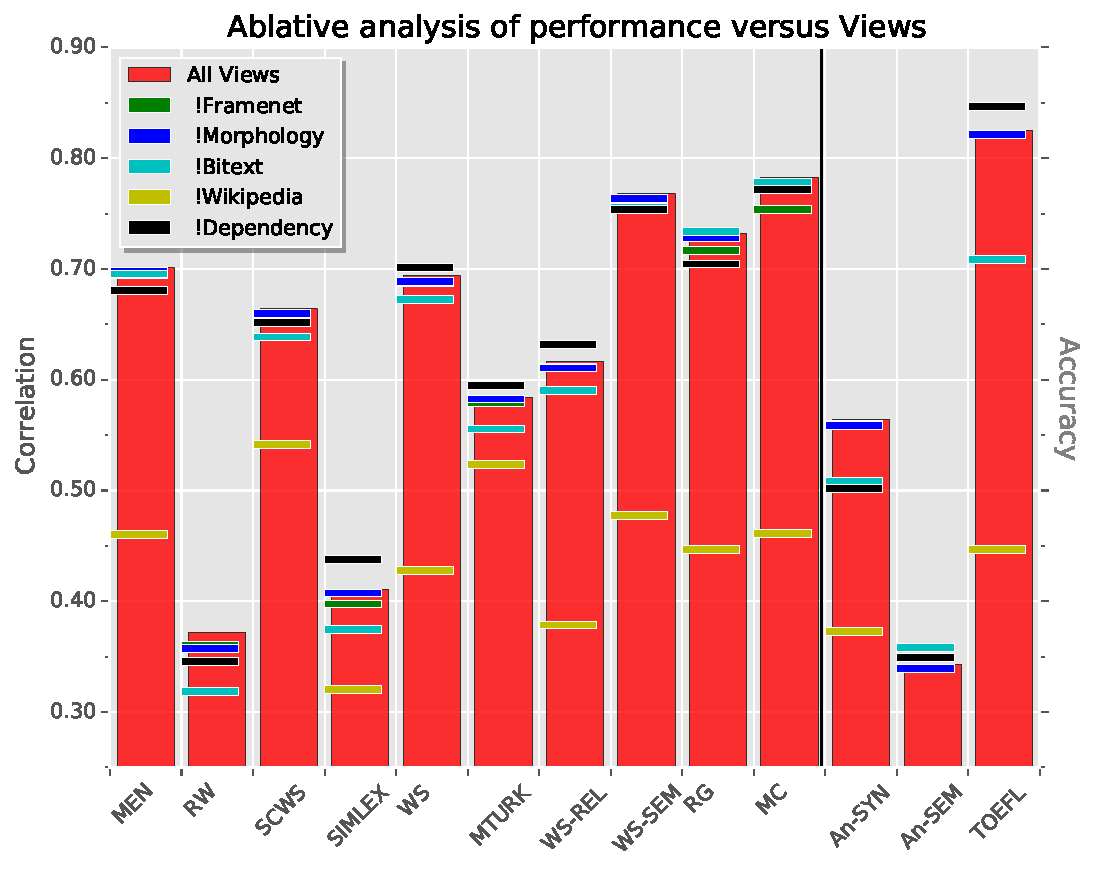
\includegraphics[width=\linewidth]{ablative_figure.pdf}
        \end{figure}
        \vspace{-0.2in}
        \begin{figure}
        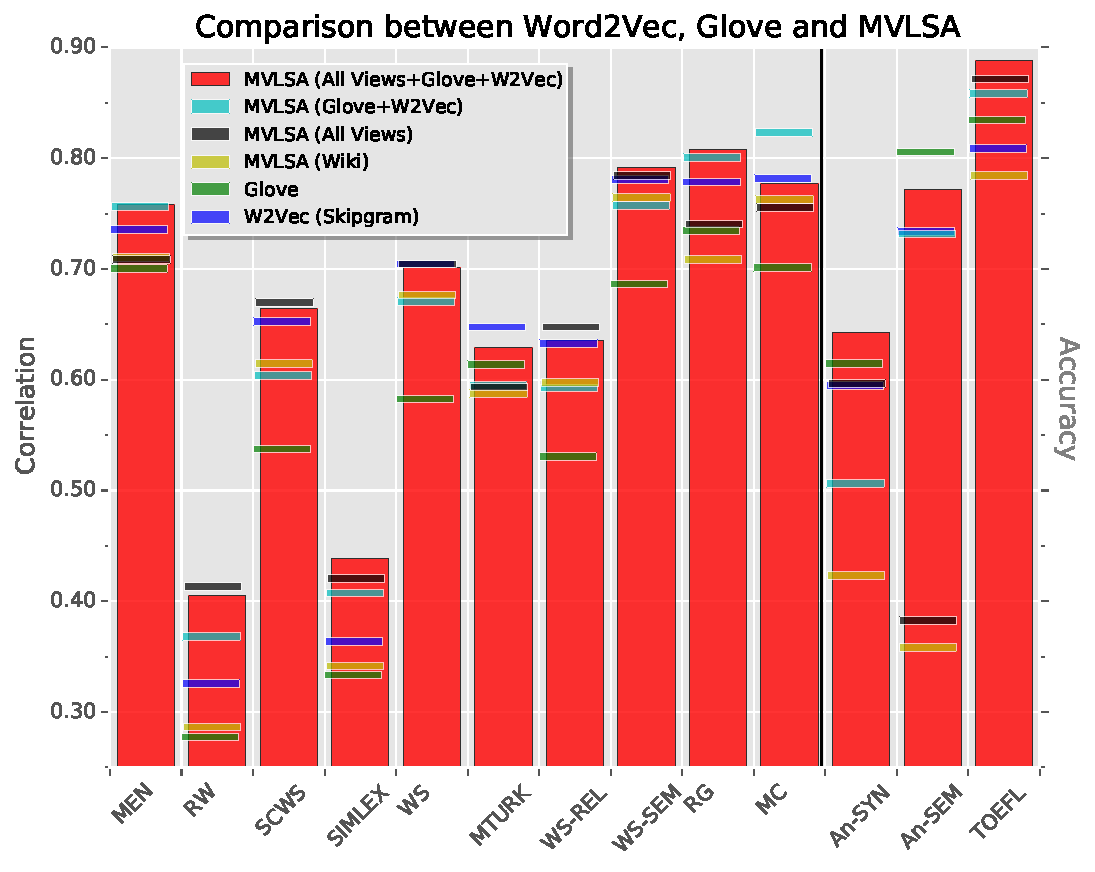
\includegraphics[width=\linewidth]{comparative_figure.pdf}
        \end{figure}
      \end{column}
    \end{columns}
  \end{column}
\end{column}
%--- END OF THE SECOND COLUMN -------
\begin{column}{\sepwid}\end{column} 
%--- START THE THIRD COLUMN ---------
\begin{column}{\onecolwid}\vspace{-0.4in}
  \begin{alertblock}{Unifying Prior Work}
    We could approximately mimic the objective of
    \cite{pennington2014glove} by changing the reweighting terms in
    our method for handling missing values as follows:
    \begin{eqnarray}
      \label{eq:gcca3}
      \minimize{G,U_j}{\sum_{j=1}^J \begin{Vmatrix} W_j K_j(G - X_jU_j) \end{Vmatrix}^2_F}{G^\top G = I }
    \end{eqnarray}

    where
    \begin{eqnarray}
      [W_j]_{ii} &=& \left(\frac{w_i}{w_{\max}}\right)^{\frac{3}{4}} \text{ if } w_i <
      w_{\max} \text{ else } 1, \nonumber \\
      \text{and } w_i &=&  \sum_k [X_j]_{ik}. \nonumber
    \end{eqnarray}
  \end{alertblock}
  %% a small set of overlapping square grids, representing matrices, having
  %% an arrow that points to a single matrix
  \begin{figure}
    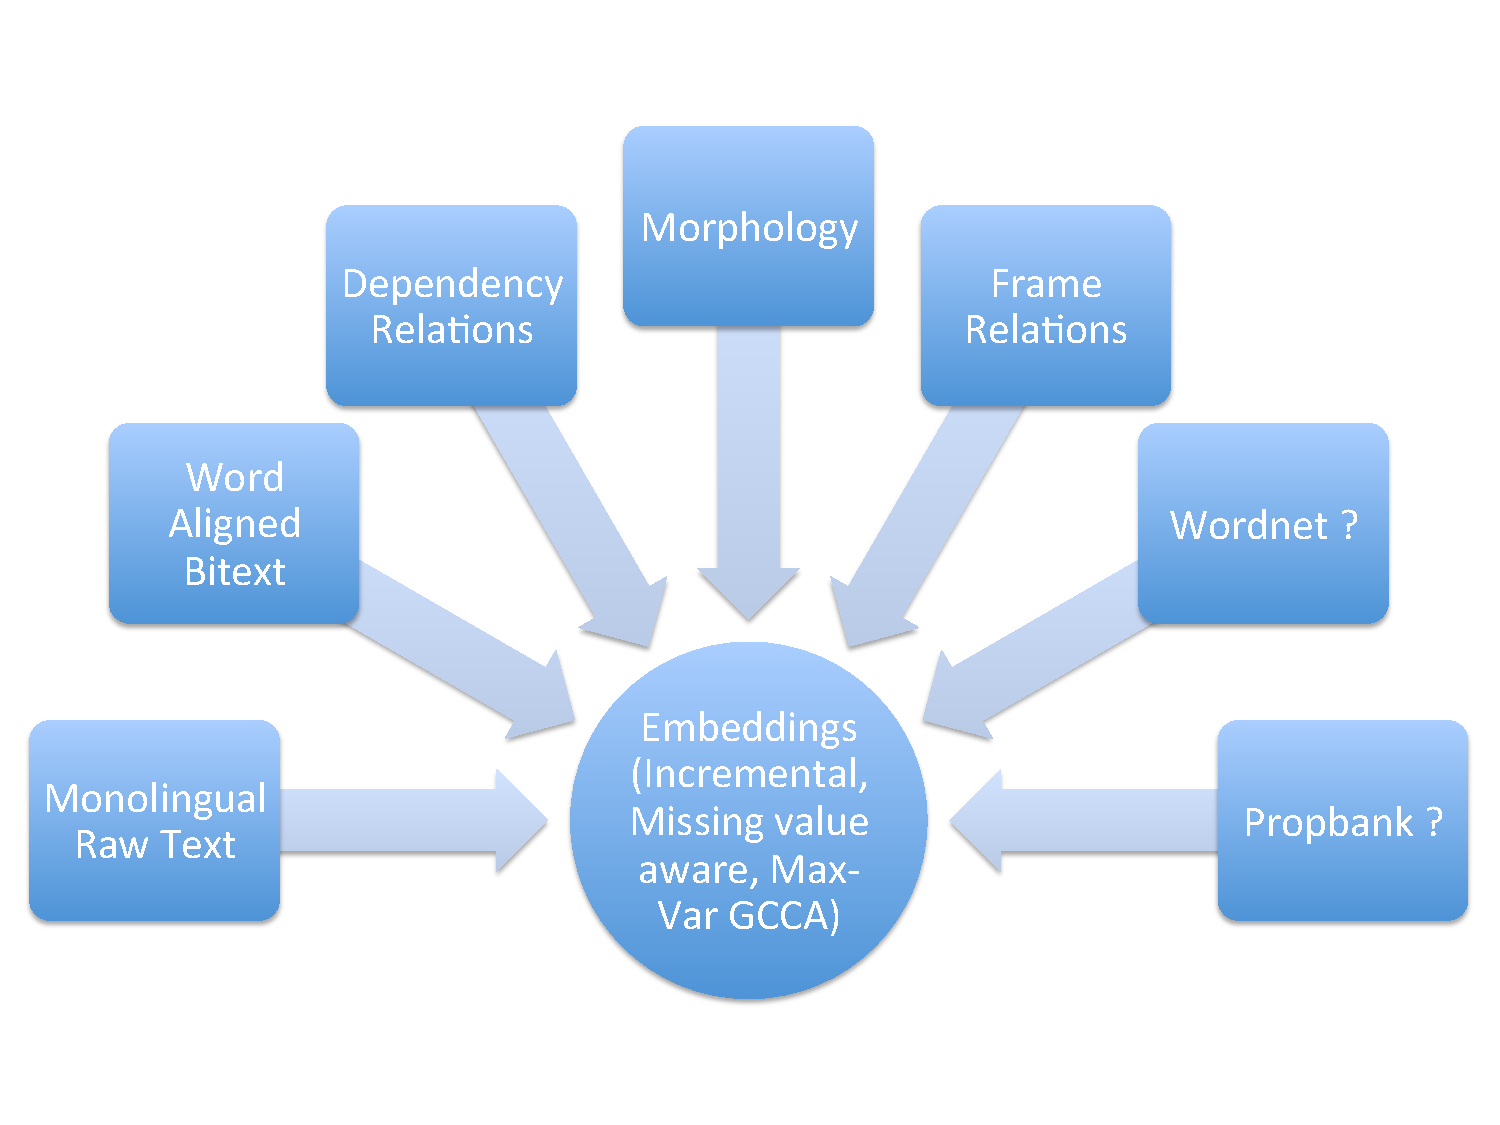
\includegraphics[trim=0 0 0 35,clip,width=\linewidth]{cartoon.pdf}
  \end{figure}

  \begin{block}{References}
    % \nocite{*} % Insert publications even if they are not cited in the poster
    \small{\bibliographystyle{abbrv}
      \bibliography{../references}}
  \end{block}

  \setbeamercolor{block alerted title}{fg=black,bg=norange}
  \setbeamercolor{block alerted body}{fg=black,bg=white}
  
    \setbeamercolor{block title}{fg=red,bg=white}
  \begin{block}{Acknowledgements}
    \small{\rmfamily{This material is based on research sponsored by Defense Advanced Research
        Projects Agency (DARPA) under the Deep Exploration and
        Filtering of Text (DEFT) Program (Agreement number
        FA8750-13-2-0017).}}
  \end{block}

\end{column}

\end{columns}
\end{frame}
\end{document}
